
\section{Тест производительности}

Для тестов я использвал утилиту gnuplot для построения графиков зависимости времени работы программы от количества чисел. Так же для сравнения использовал библиотеку chrono для замера времени.

\begin{figure}[h]
  \begin{center}
    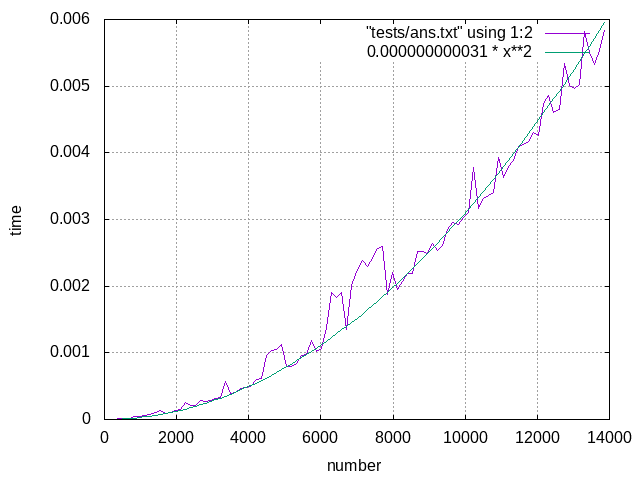
\includegraphics[scale=0.5]{../plots/plot1.png}
  \end{center}
  \caption{Графики работы жадного алгоритма и сопоставление с квадратичной функцией}
\end{figure}

\begin{figure}[h]
  \begin{center}
    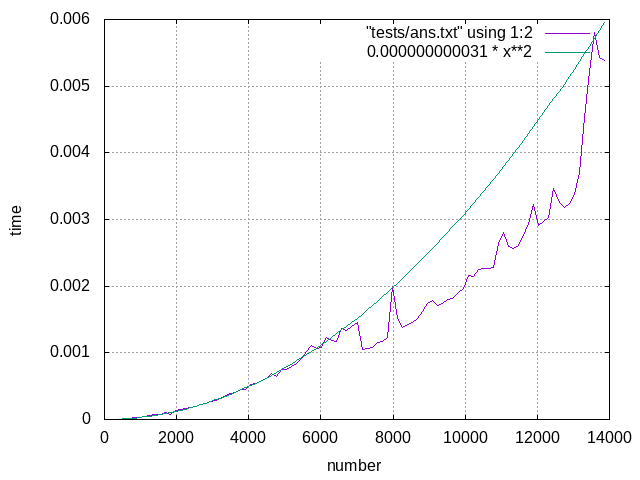
\includegraphics[scale=0.5]{../plots/plot.png}
  \end{center}
  \caption{Графики работы жадного алгоритма без обмена во втором блоке и сопоставление с квадратичной функцией из прошлого примера}
\end{figure}

Как видно сложность алгоритмов одинаковая и в худшем случае второй приближается к первому.

\pagebreak
